\documentclass[hidelinks,a4paper,11pt, nofootinbib]{article}
\usepackage[left=2cm, top=2.5cm, right=2cm, width=15.5cm, height= 24.5cm]{geometry}
\usepackage[spanish, es-tabla]{babel} %es-tabla es para que ponga Tabla en vez de Cuadro en el caption
\usepackage[utf8]{inputenc}
\usepackage[T1]{fontenc}
\usepackage{xspace}
\usepackage{xargs}
\usepackage{fancyhdr}
\usepackage{lastpage}
\usepackage{caratulaMetNum}
\usepackage[bottom]{footmisc}
\usepackage{amssymb}
\usepackage{algorithm}
\usepackage[noend]{algpseudocode}
\usepackage{array}
\usepackage{xcolor,colortbl}
\usepackage{rotating}
\usepackage{lscape}

\usepackage{pgf}
\usepackage{tikz}
\usetikzlibrary{arrows,automata}

\usepackage{graphicx}
\usepackage{sidecap}
\usepackage{amsmath}
\usepackage{wrapfig}
\usepackage{caption}

\usepackage{hyperref}
\hypersetup{
  colorlinks   = true, %Colours links instead of ugly boxes
  urlcolor     = blue, %Colour for external hyperlinks
  linkcolor    = blue, %Colour of internal links
  citecolor   = red %Colour of citations
}

\usepackage{comment}

\usepackage[
  backend=bibtex,
  style=alphabetic
]{biblatex}
\addbibresource{bibliografia.bib}


\captionsetup[table]{labelsep=space}


\setlength{\parindent}{4em}
\setlength{\parskip}{0.5em}

%Defino colores para las tablas
\definecolor{LightCyan}{rgb}{0.77,0.9,0.9}
\definecolor{Gray}{gray}{0.8}
\DeclareMathOperator*{\argmin}{arg\,min}

%%fancyhdr
\pagestyle{fancy}
\thispagestyle{fancy}
\addtolength{\headheight}{1pt}
\lhead{Métodos Numéricos: TP3}
\rhead{$2º$ cuatrimestre de 2015}
\cfoot{\thepage\ / \pageref{LastPage}}
\renewcommand{\footrulewidth}{0.4pt}

%%caratula
\materia{Laboratorio de Métodos Numéricos}
\titulo{Trabajo Práctico Número 3}
\subtitulo{\emph{Un juego de niños}}
%\grupo{Grupo 12}
\integrante{Ciruelos Rodríguez, Gonzalo}{063/14}{gonzalo.ciruelos@gmail.com}
\integrante{Costa, Manuel José Joaquín}{035/14}{manuc94@hotmail.com}
\integrante{Gatti, Mathias Nicolás}{477/14}{mathigatti@gmail.com}

\abstracto{En el presente trabajo práctico nos proponemos atacar el problema de incrementar la cantidad de cuadros de un video con el fin de obtener un efecto de cámara lenta o simplemente mejorar la fluidez del mismo. Para esto consideramos un modelo matemático de la situación que nos permite llevar el problema al terreno de la interpolación. Una vez hecho esto, resolveremos el nuevo problema haciendo uso de tres métodos ampliamente conocidos en el área: vecino más cercano, interpolación lineal y trazadores cúbicos (o splines cúbicos). A su vez para el método de splines consideraremos tres variantes, modificando el tamaño del bloque usado, es decir la cantidad de \textit{frames} originales de los que dependerán los \textit{frames} interpolados. Evaluaremos las ventajas y desventajas de cada uno en términos de tiempo de cómputo, fiabilidad (por ejemplo, trataremos de minimizar los \textit{artifacts}) y fluidez de los resultados obtenidos.
Para esto consideraremos distintos tipos de videos que exploten diversas características (por exceso o defecto) como son movimientos de cámara, movimientos abruptos de objetos, etc. Finalmente, concluiremos que en términos generales la interpolación lineal y los splines cúbicos con bloques de tamaño ocho son los que nos dan las mejores prestaciones según la situación.}

\palabraClave{Cámara lenta}
\palabraClave{Vecino más cercano}
\palabraClave{Interpolación lineal}
\palabraClave{Splines cúbicos}

\usepackage{etoolbox}
\AtBeginEnvironment{tikzpicture}{\shorthandoff{>}\shorthandoff{<}}{}{}

\begin{document}
\maketitle

\tableofcontents
\newpage

\section{Introducción teórica}
El objetivo del presente informe es resolver un problema práctico mediante el modelado matemático del mismo. Este problema consiste en generar videos en camará lenta dados los videos originales, utilizando métodos de interpolación numérica.

Por lo tanto, vamos a tener que colocar más cuadros entre cada par de cuadros consecutivos del video original. Para esto, vamos a pensar un pixel del video a lo largo de todos los frames.
\[p_{ij}(f)\]

Donde el pixel (ij-ésimo) de un video depende del frame. Entonces, la idea va a ser interpolar esta función para obtener los potenciales valores intermedios. 

Entonces, por ejemplo, si tenemos un video de 1x1 píxeles, y los valores

\[ p_{11}(0), p_{11}(1), ..., p_{11}(n)\]

Si nos piden colocar 2 nuevos frames entre cada frame viejo, vamos a estar interesado en los valores

\begin{center}
\begin{tabular}{c}
$p_{11}\left(0\right), p_{11}\left(\frac13\right), p_{11}\left(\frac23\right), p_{11}\left(1\right), p_{11}\left(\frac43\right), p_{11}\left(\frac53\right), p_{11}\left(2\right), ...,$ \\
$p_{11}\left(n-1\right), p_{11}\left(n- \frac23\right), p_{11}\left(n- \frac13\right), p_{11}\left(n\right)$ \\
\end{tabular}
\end{center}

Entonces la idea es fijar un algoritmo de interpolación y obtener todos esos valores, para luego poder rearmar el video.

Estos métodos, además de permitirnos realizar cámaras lentas, también permiten realizar interpolación para otros fines.
Por ejemplo, al streamear un video, podríamos bien no recibir todos los cuadros del video, y que el reproductor los interpole acordemente para generar un video fluido. Otro ejemplo de uso es una cámara -- de mala calidad -- que no puede filmar a 24 cuadros por segundo, pero que sin embargo con estos algoritmos, a partir de videos de menor framerate, podemos generear videos fluidos.


\newpage

\section{Desarrollo}
\subsection{Convenciones}



\subsection{Métodos numéricos usados}

Como dijimos en la introducción, nuestro objetivo será, dada una lista de valores que toma un pixel a lo largo de diferentes frames, obtener una función que los interpole y luego usarla para obtener valores intermedios.

Dados,

\[ p_0, p_1, p_2, ..., p_n \]

Queremos obtener \[p_{ij}(f) \]

Tal que \[p_{ij}(0) = p_0, p_{ij}(1) = p_1, p_{ij}(2) = p_2, ..., p_{ij}(n) = p_n\]

Y el resto de los valores intermedios se obtienen usando $p_{ij}$. Entonces, si nos piden colocar $k$ cuadros entre 2 cuadros existentes (supongamos cuadro 0 y cuadro 1 por simplicidad), debemos computar los siguientes valores:

\[p_{ij}\left(\frac1{k+1}\right), p_{ij}\left(\frac2{k+1}\right), p_{ij}\left(\frac3{k+1}\right), ..., p_{ij}\left(\frac{k}{k+1}\right)\]

Y análogamente para el resto de los cuadros.

Ahora pasemos a ver los métodos implementados y analizados en este trabajo.


\subsubsection{Vecino más cercano}

El primer método, llamado vecino más cercano o \emph{nearest neighbour} en inglés, se basa en interpolar un punto por el valor del punto más cercano conocido. Formalmente, si $(x_1, y_1), ..., (x_n, y_n)$ son nuestros puntos de dato, la función que interpola sería:

\[ f(x) = f(\argmin_{i} |x - x_i|) \]
\[ f(x_i) = y_i \]

En el caso particular de este problema, es más simple aún. Si tenemos que colocar $k$ cuadros entre 2 cuadros consecutivos $c_1$ y $c_2$, simplemente podemos poner $\frac{k}{2}$ cuadros con el valor de $c_1$ y luevo $\frac{k}{2}$ cuadros con el valor de $c_2$.


En el caso de que $k$ sea impar, simplemente tenemos un valor en el medio al que podemos darle cualquiera de los 2 valores, es una decisión de diseño. En el caso de este trabajo, ese valor es $c_2$


\subsubsection{Interpolación lineal}

La interpolación lineal (de a trozos) es la interpolación polinomial de a trozos más simple. Consiste en unir una serie de puntos

\[ (x_0, f(x_0)), (x_1, f(x_1)), (x_2, f(x_2)), ..., (x_n, f(x_n)) \]

por lineas rectas. Una desventaja de este método, como analizaremos en la experimentación, es que no necesariamente la función resultante va a ser diferenciable en los $x_i$, algo generalmente deseable, sobre todo en este caso en que la no diferenciabilidad se vería reflejada en cambios bruscos en el video.

En general, dados los puntos $(x_i, f(x_i)), (x_{i+1}, f(x_{i+1}))$, si queremos interpolarlos con una recta obtenemos

\[ l_i(x) = f(x_i) + \frac{f(x_{i+1}) - f(x_i)}{x_{i+1} - x_i} (x - x_i) \]

Entonces, el algoritmo se basa en esa fórmula, evaluándola en los puntos que se nombraron anteriormente.

\subsubsection{Splines cúbicos}

Los splines cúbicos son una interpolación polinómica (cúbica) de a trozos, que se basa en pedirle condiciones fuertes a los polinomios cúbicos que interpolan cada trozo de la función. En el caso del spline natural, si le llamamos $S_i$ al $i$ésimo spline cubico,

\begin{enumerate}
    \item $S_i(x_i) = S_i(x_{i+1})$, es decir, que la función resultante sea continua en todo punto.
    \item $S_i'(x_i) = S_i'(x_{i+1})$, es decir, que la función resultante sea derivable en todo punto.
    \item $S_i''(x_i) = S_i''(x_{i+1})$, es decir, que la función resultante sea segundo derivable en todo punto.
    \item $S_0''(x_0) = S_{n-1}''(x_n) = 0$, porque esta es la condición del spline natural.
\end{enumerate}

Este método obviamente permite obtener como resultado una función mas apropiada, a priori, para nuestro problema, dado que la derivabilidad nos garantiza que las transiciones van a ser más suaves que con la interpolación lineal.

En el caso de este trabajo, se requirió que la cantidad de cuadros que se tienen en cuenta para hacer el spline sea fija y a elección del usuario. Analizaremos las implicaciones de esto en la experimentación.

Para una explicación más profunda del método, se puede consultar \cite{burden}. Además, la implementación de splines de este trabajo también esta basada en \cite{burden}, posee algunas correcciones y está modificada para permitir realizar la interpolación de a bloques de tamaño fijo.


\subsection{Estructuración del código}

Para el modelado del problema utilizamos una interfaz muy simple. El archivo \texttt{tp-main.cpp} se ocupa de leer el todo el input, llamar a la rutina interpoladora correspondiente para cada pixel, y luego praparar el resultado para finalmente escribirlo en el archivo de output.

Lo que hacemos es tener una variable \texttt{frames} de tipo \texttt{std::vector < std::vector<unsigned int > {} > }, en la que el vector \texttt{frames[k]} representa los valores del pixel $k$ en cada frame(pensamos al video como una tira de pixeles en lugar de una matriz de pixeles).


Entonces, simplemente, para cada $k$ entre 0 y $ancho * alto$, tenemos un vector $frames[k]$, que podemos pensar como una funcion $ k \mapsto $\texttt{frames[$k$]}; y esta función será la que interpolemos, como explicamos anteriormente.

Ahora pasaremos a describir brevemente los métodos utilizados.


\subsubsection{Nearest Neighbour}
\texttt{\textbf{vector<unsigned int>} nn(\textbf{vector<unsigned int>} valores, \textbf{int} cuadros)}

\begin{itemize}
    \item  \underline{valores} será, como dijimos antes, \texttt{frames[$k$]}, para algun $k$.
    \item \underline{cuadros} serán la cantidad de valores nuevos a colocar entre dos valores consecutivos de \underline{valores}.
\end{itemize}

El código es muy simple, y respeta lo explicado anteriormente cuando se describió el método


\subsubsection{Interpolación Lineal Fragmentaria}
\texttt{\textbf{vector<unsigned int>} lineal(\textbf{vector<unsigned int>} valores, \textbf{int} cuadros)}

\begin{itemize}
    \item  \underline{valores} será \texttt{frames[$k$]}, para algun $k$.
    \item \underline{cuadros} serán la cantidad de valores nuevos a colocar entre dos valores consecutivos de \underline{valores}.
\end{itemize}


Como dijimos anteriormente, la interpolación lineal fragmentaria se basa en, dados los puntos $(a,f(a)), (b,f(b))$, interpolar entre ellos con \[\frac{f(b)-f(a)}{b-a} (x-a) + f(a)\]

En este caso, la formula para un $k$ dado sería,

\[\frac{valores[k+1] - valores[k]}{k+1 - k} (x - k) + valores[k] = (valores[k+1] - valores[k]) (x - k) + valores[k] \]

Entonces, hacemos como explicamos anteriormente, y en el caso de que $cuadros = c$, basta con tomar los siguientes valores para $x - k$:

\[\frac1{c+1}, \frac2{c+1}, ..., \frac{c}{c+1}\]

\subsubsection{Splines cúbicos}

\texttt{\textbf{vector<unsigned int>} splines(\textbf{vector<unsigned int>} valores, \textbf{int} cuadros, \textbf{int} radio)}

\begin{itemize}
    \item  \underline{valores} será \texttt{frames[$k$]}, para algun $k$.
    \item \underline{cuadros} serán la cantidad de valores nuevos a colocar entre dos valores consecutivos de \underline{valores}.
    \item \underline{radio} será la cantidad de cuadros que contendrá cada bloque. No es necesario que radio divida a la cantidad de cuadros, en ese caso el ultimo bloque simplemente tendrá menos cuadros (sí es necesario que el último bloque tenga más de 3 cuadros, para poder resolver el sistema).
\end{itemize}

La función splines simplemente lo que hace es partir al video en bloques, y para cada bloque generar el spline correspondiente e interpolar allí utilizandolo. Para llevar esto a cabo, se utilizará la funcion:


\texttt{\textbf{void} splines\_bloque(vector<double> ys, \textbf{int} cuadros, \textbf{vector<double>*} resultado)}

Esta función se ocupará de obtener el spline que interpola a los valores de \textbf{ys} utilizando el algoritmo de \cite{burden} modificado para que funcione correctamente. Luego, hara \textbf{push\_back} de los resultados en  \textbf{resultado}.




\subsection{Experimentación}

La experimentación del presente trabajo se divide a grandes rasgos en tres partes:

\begin{itemize}
    \item Primero nos ocuparemos de las mediciones de tiempos y análisis de complejidad de los algoritmos y métodos utilizados.
    \item Luego, nos centraremos en lo que concierne la medición del error de los resultados obtenidos a partir de los métodos, desde un punto de vista cuantitativo.
    \item Finalmente, nos centraremos en un análisis cualitativo de los resultados, intentando analizar subjetivamente los resultados obtenidos, especialmente buscando \emph{artifacts} o errores que la simple medición del error numérico no nos permite percibir.
\end{itemize}

En cada parte explicaremos la metodología con la que realizamos los experimentos correspondientes, además de analizar en profundidad los resultados obtenidos.





\newpage

\section{Resultados y discusión}
\subsection{Análisis de rendimiento}
A continuación realizaremos un análisis de los tiempos insumidos por los métodos, el cual estará dividido en dos partes: primero, en forma preliminar para tener una orientación de que variables estudiar, un análisis superficial de la complejidad algorítmica de cada método; y luego, la contrastación empírica.

La PC sobre la que se tomaron los tiempos cuenta con un procesador Intel(R) Core(TM) i5-2500 @ 3.30GHz y 8GB de RAM.

\subsubsection{Complejidades de los métodos}
Utilizaremos la siguiente notación:
\begin{itemize}
	\item $cuadros\_originales$: la cantidad de cuadros que tiene el video original.
	\item $pixeles$: la cantidad de píxeles que tiene cada \emph{frame} del video.
	\item $cuadros$: la cantidad de cuadros que se desea agregar entre los existentes del video original.
\end{itemize}

En el caso de \emph{nearest neighbour} es bastante fácil darse cuenta que la complejidad es 

\begin{center}
	$O(cuadros\_originales \times pixeles \times cuadros)$
\end{center}

pues por cada píxel de cada cuadro copiamos $cuadros$ píxeles (lo que nos cuesta $O(1)$).

Para interpolación lineal pasa más o menos lo mismo, con la diferencia de que en lugar de copiar el píxel realiza unas pocas operaciones básicas que no dejan de ser $O(1)$, por lo que su complejidad es igual a la anterior.

Para analizar splines, vamos a considerar la partición en $n$ bloques de tamaño $b_1,..., b_n$ (o sea, ni siquiera suponemos que todos los bloques sean del mismo tamaño). Como por cada píxel se llama a la función \texttt{splines}, simplemente calculemos su complejidad y luego la multiplicamos por $pixeles$.

El costo de \texttt{splines} es la sumatoria de los costos de llamar a \texttt{splines\_bloque} por cada bloque. La complejidad de esta última función es 
\begin{center}
	$O(b\_i + b\_i \times cuadros) = O(b\_i \times cuadros)$
\end{center}

pues primero se resuelve el sistema con costo lineal \footnote{la complejidad exacta del algoritmo usado para resolver el sistema tridiagonal puede encontrarse en el capítulo 6 de \cite{burden}} sobre el tamaño del bloque, y luego por cada elemento del bloque se realizan $cuadros$ iteraciones de costo $O(1)$. Entonces nos queda que la complejidad de \texttt{splines} es

\begin{equation*}
\begin{split}
b_1 \times cuadros + b_2 \times cuadros + ... + b_n \times cuadros & = cuadros \times (b_1 + ... + b_n) \\
& = cuadros \times cuadros\_originales
\end{split}
\end{equation*}

Como esto había que multiplicarlo por $pixeles$, la complejidad total del método termina siendo igual a la de los dos métodos anteriores, aunque en este caso las constantes que se están ignorando son más significativas.

De esto deducimos entonces que las variables a analizar en la experimentación deben ser $cuadros$,  $cuadros\_originales$ y $pixeles$ (es decir, la resolución del video).

\subsubsection{Cantidad de cuadros a agregar}
Para esta sección consideramos variaciones con menos cuadros (para poder experimentar con mayor comodidad) de tres videos:
\begin{itemize}
	\item ff6: Versión de 22 cuadros, resolución 400x225
	\item darthvader: Versión de 15 cuadros, resolución 400x225
	\item penal: Versión de 18 cuadros, resolución 560x315
\end{itemize}

En base a los resultados de la sección anterior, es de esperar que para todos los métodos el tiempo de cómputo sea lineal sobre la cantidad de cuadros que se desean agregar. Sin embargo, está claro que las pendientes de cada método serán distintas pues las constantes lo son.  
Las hipótesis son realitavemente obvias: el método de vecino más cercano será el más veloz pues no realiza ningún cáculo sino que simplemente copia píxeles; lineal será el segundo más rápido pues a diferencia del anterior se agrega el cálculo de un polinomio de grado 1. Claramente los splines serán los que más tarden pues requieren evaluar un polinomio de grado 3 por cada cuadro a agregar. A su vez, es de esperar que independientemente del tamaño de bloque considerado para splines (4, 8 o 12), el tiempo de cómputo sea el mismo. Esto es consecuencia inmediata de que la complejidad del método, como vimos en la sección anterior, no depende de la partición escogida.


A continuación presentamos los resultados. Los mismos se obtuvieron de realizar 20 iteraciones para cada método y cantidad de cuadros a agregar.
\begin{figure}[H]
 \centering
	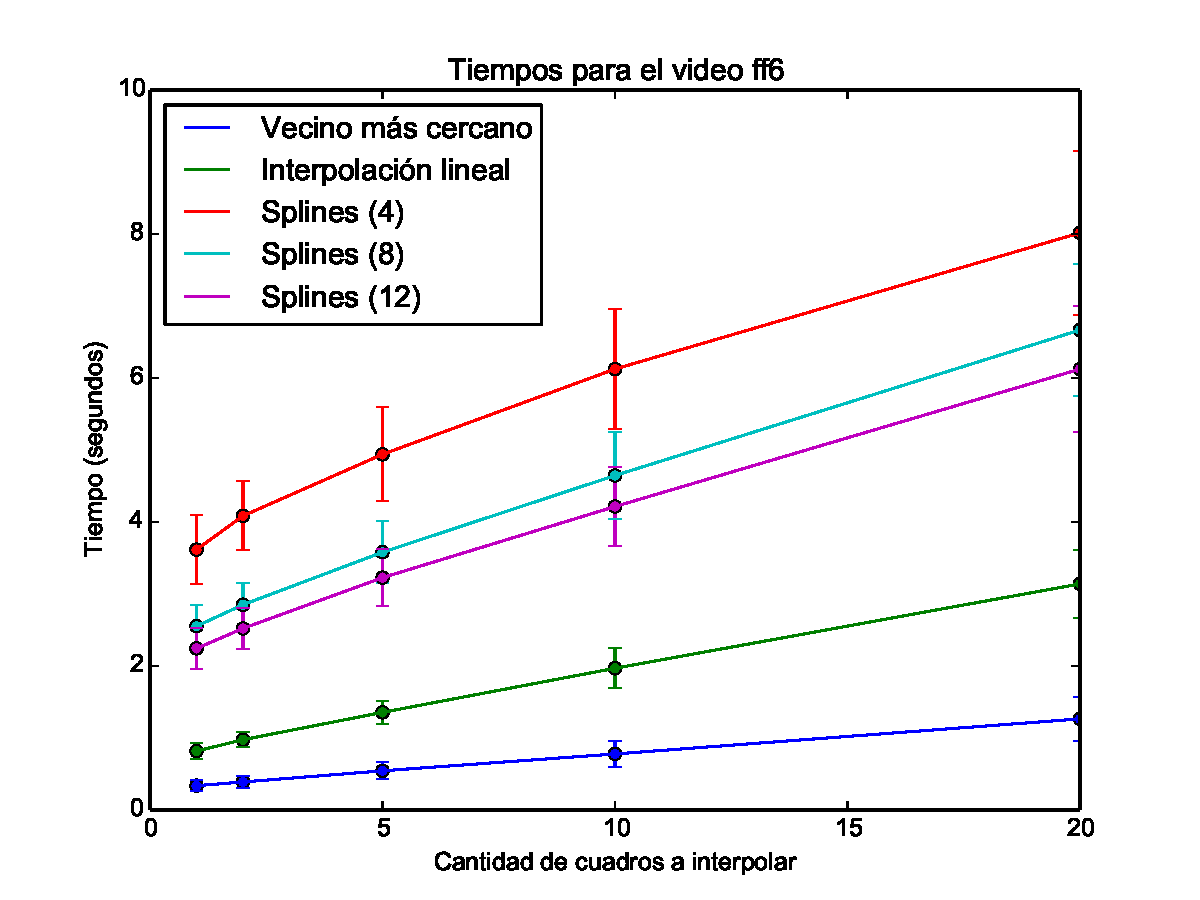
\includegraphics[width=0.7\textwidth]{imgs/resultados_tiempos/ff6_times.pdf}
	\caption{\footnotesize Tiempo que cuesta aplicar cada método sobre ff6 en función de la cantidad de cuadros que se desean agregar. Los puntos representan la media 0.20-podada de cada muestra. Las barras verticales indican la varianza.}
	\label{fig:ff6-times}
\end{figure}

\begin{figure}[H]
 \centering
	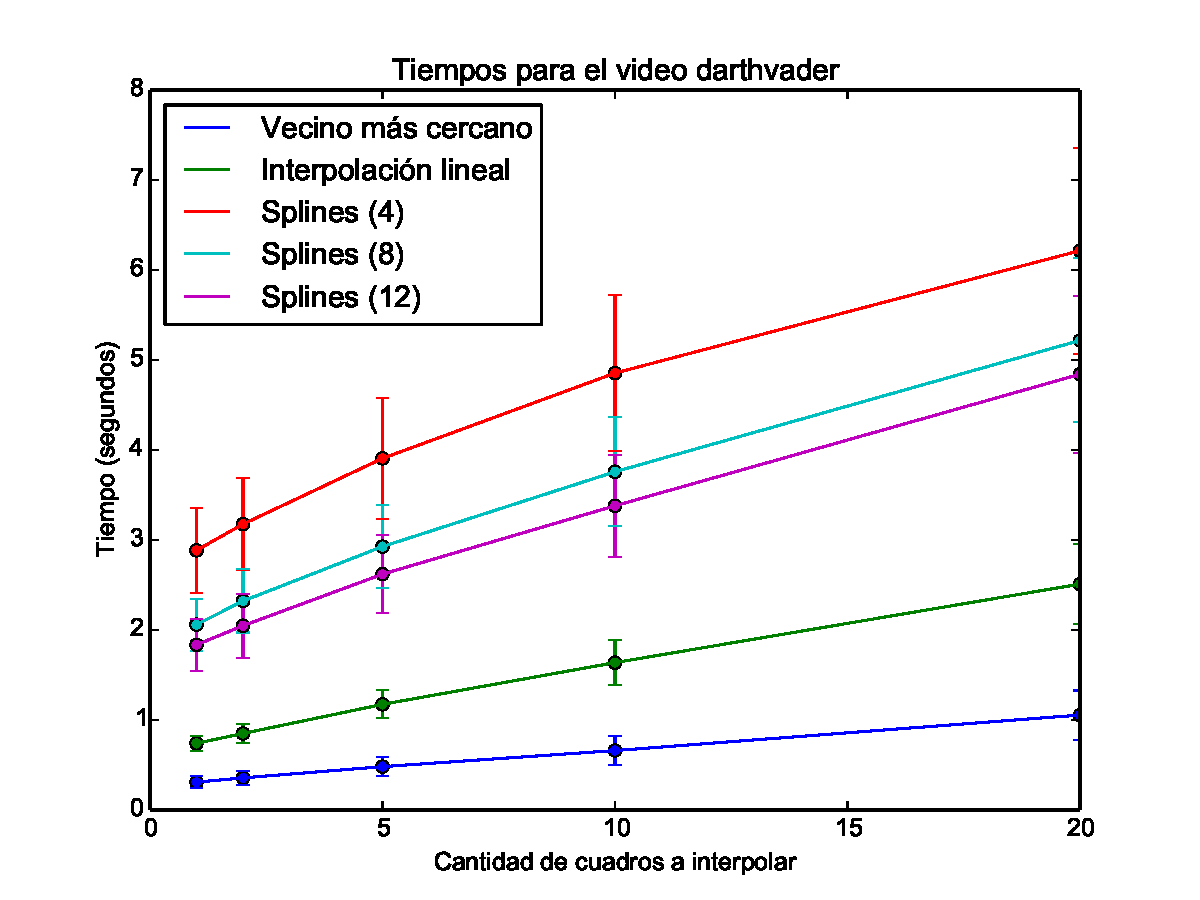
\includegraphics[width=0.7\textwidth]{imgs/resultados_tiempos/darthvader_times.pdf}
    \caption{\footnotesize Tiempo que cuesta aplicar cada método sobre darthvader en función de la cantidad de cuadros que se desean agregar. Los puntos representan la media 0.20-podada de cada muestra. Las barras verticales indican la varianza.}
    \label{fig:darthvader-times}
\end{figure}

\begin{figure}[H]
 \centering
	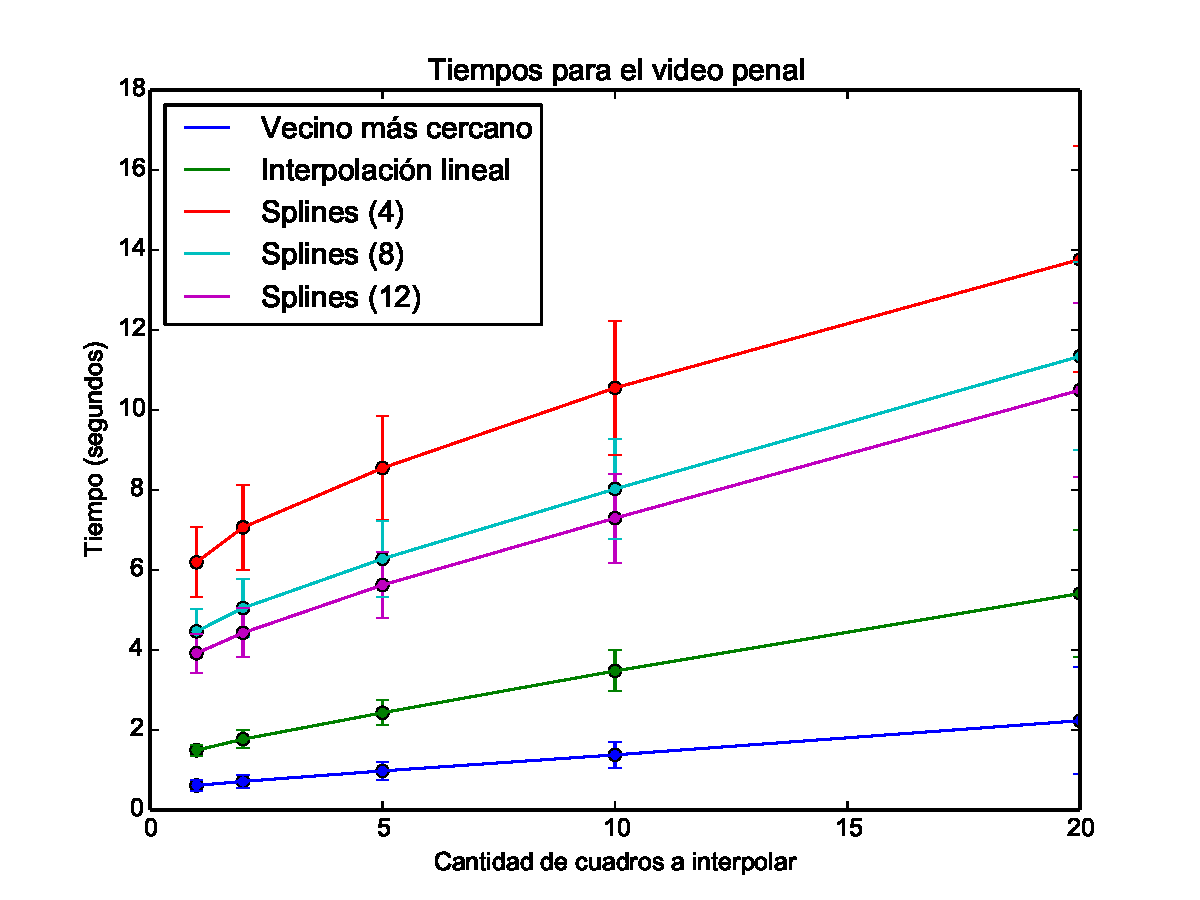
\includegraphics[width=0.7\textwidth]{imgs/resultados_tiempos/penal_times.pdf}
    \caption{\footnotesize Tiempo que cuesta aplicar cada método sobre penal en función de la cantidad de cuadros que se desean agregar. Los puntos representan la media 0.20-podada de cada muestra. Las barras verticales indican la varianza.}
    \label{fig:penal-times}
\end{figure}

Al ver los gráficos vemos que se sostienen las hipótesis respecto de los métodos de vecino más cercano e interpolación lineal, pero curiosamente las tres variantes de splines muestran tiempos distintos. No solo eso, sino que consistentemente en todos los casos a mayor tamaño de bloque, menos tarda en computar el método.

Si observamos con un poco más de detenimiento las figuras \ref{fig:darthvader-times} y \ref{fig:penal-times} vemos que las varianzas de los splines son altas y en muchos casos se superponen las tres, pero la figura \ref{fig:ff6-times} que muestra una varianza un poco más acotada parece señalar que la tendencia marcada en el párrafo anterior efectivamente existe. Parece razonable atribuirle gran parte de esto al hecho de que, al considerar particiones de bloques más pequeños, se llama más veces a la función  \texttt{splines\_bloque} y se entra más al ciclo \texttt{while} de \texttt{splines}, lo que provoca que las constantes que despreciamos al calcular la complejidad incidan más en la brecha de tiempos observada. Más específicamente, son las constantes que sumaban las que provocan la diferencia, pues al ver el gráfico vemos que lo que ocurre es un corrimiento sobre el eje de ordenadas pero no un cambio de curvatura.


\subsubsection{Tamaño de bloque}
Las hipótesis son escencialmente análogas al caso anterior. Ahora con la corrección de que seguramente veamos un fenómeno similar al visto antes con respecto a los tres métodos de splines.

\begin{figure}[H]
 \centering
	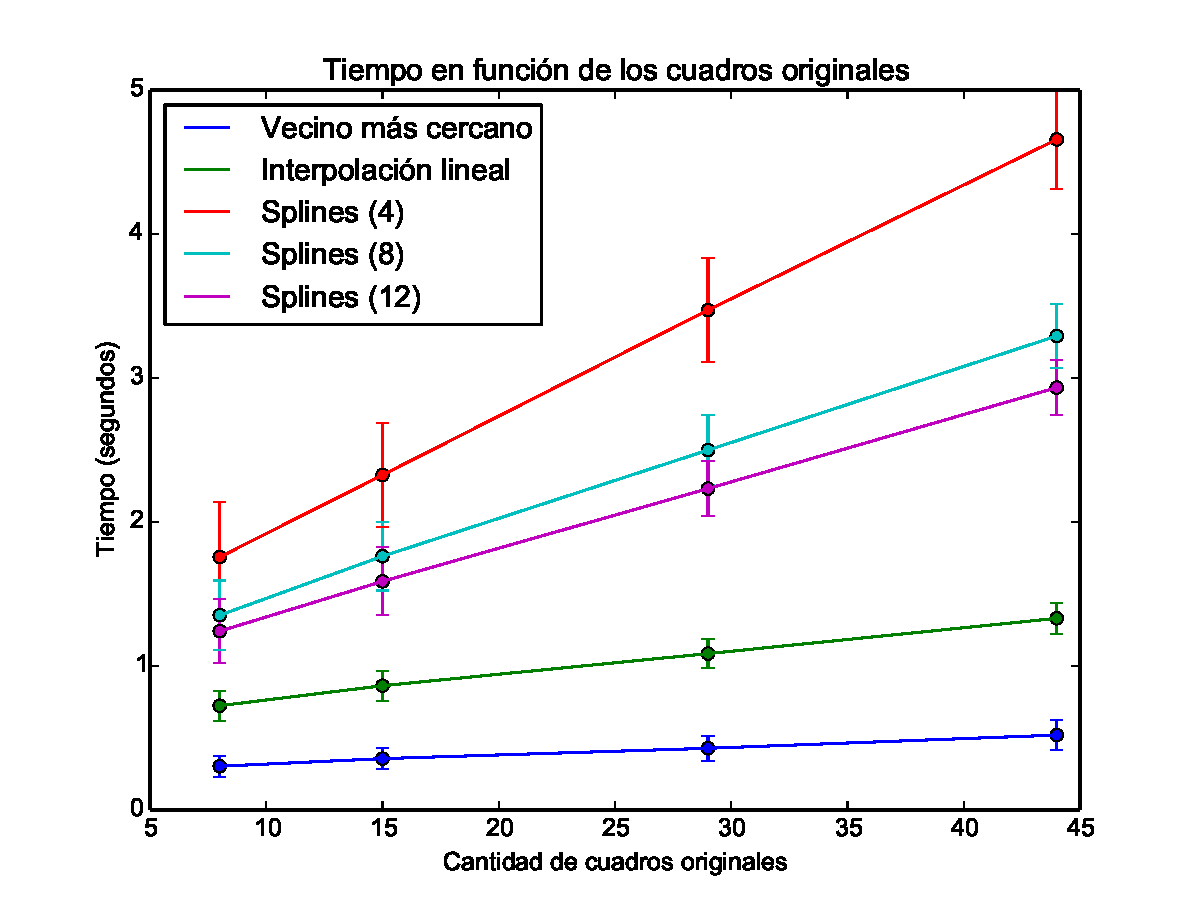
\includegraphics[width=0.7\textwidth]{imgs/resultados_tiempos/ff6_times_cuadros.pdf}
	\caption{\footnotesize Tiempo que se requiere al aplicar cada método sobre un video para interpolar 2 cuadros en función de la cantidad de cuadros que poseía originalmente. Los puntos representan la media 0.20-podada de cada muestra. Las barras verticales indican la varianza.}
	\label{fig:ff6-times-cuadros}
\end{figure}

La figura \ref{fig:ff6-times-cuadros} efectivamente corrobora lo esperado. 

Algo interesante que puede observarse en este gráfico es que, a diferencia de lo que pasaba al aumentar los cuadros a agregar, las pendientes con las que crecen las curvas de las tres variantes de splines no son iguales. Es decir, en las figuras de la \ref{fig:ff6-times} a la \ref{fig:penal-times} puede apreciarse que la curvatura de los puntos es prácticamente igual aunque haya un desplazamiento sobre el eje de ordenadas. Sin embargo, aquí vemos que los puntos correspondientes a la versión que usa bloques de tamaño 4 están cada vez más espaciados de los otros. Incluso entre los correspondientes a \emph{splines (8)} y \emph{splines (12)} puede notarse esta diferencia de pendiente aunque en menor medida.

Esto resulta razonable a la luz de los hechos vistos en el punto anterior: si habíamos dicho que el tiempo del método aumentaba cuantas más veces se caía en el \texttt{while} de la función \texttt{splines} es lógico que al aumentar la variable de la cual este hecho depende directamente esta situación se potencie. Visto con un ejemplo: si dado un video le aumentáramos en 8 la cantidad de sus cuadros originales, para \emph{splines (8)} y \emph{splines (12)} esto implicaría a lo sumo caer una vez más en el \texttt{while}, mientras que para \emph{splines (4)} resulta en hacerlo dos veces más. Si lo hiciéramos en 24 cuadros, serían 2 veces para \emph{splines (12)}, 3 para \emph{splines (8)} y 6 para \emph{splines (4)}. Es decir que el aumento siempre es desigual, y eso justifica la diferencia en las pendientes.

\subsubsection{Resolución}
Finalmente, analicemos la influencia de la resolución. Es de suponer que el comportamiento sea similar al del caso anterior, o sea, que las pendientes de crecimiento sean distintas para todos los métodos, pues la cantidad de píxeles que conforman un \emph{frame} es lo que determina la cantidad de veces que se llame a las funciones que implementan los métodos de interpolación, por lo cual es razonable que todas las constantes propias de cada método se vean potenciadas.

En efecto, la figura \ref{fig:times-resolucion} verifica estas suposiciones.  

\begin{figure}[H]
 \centering
	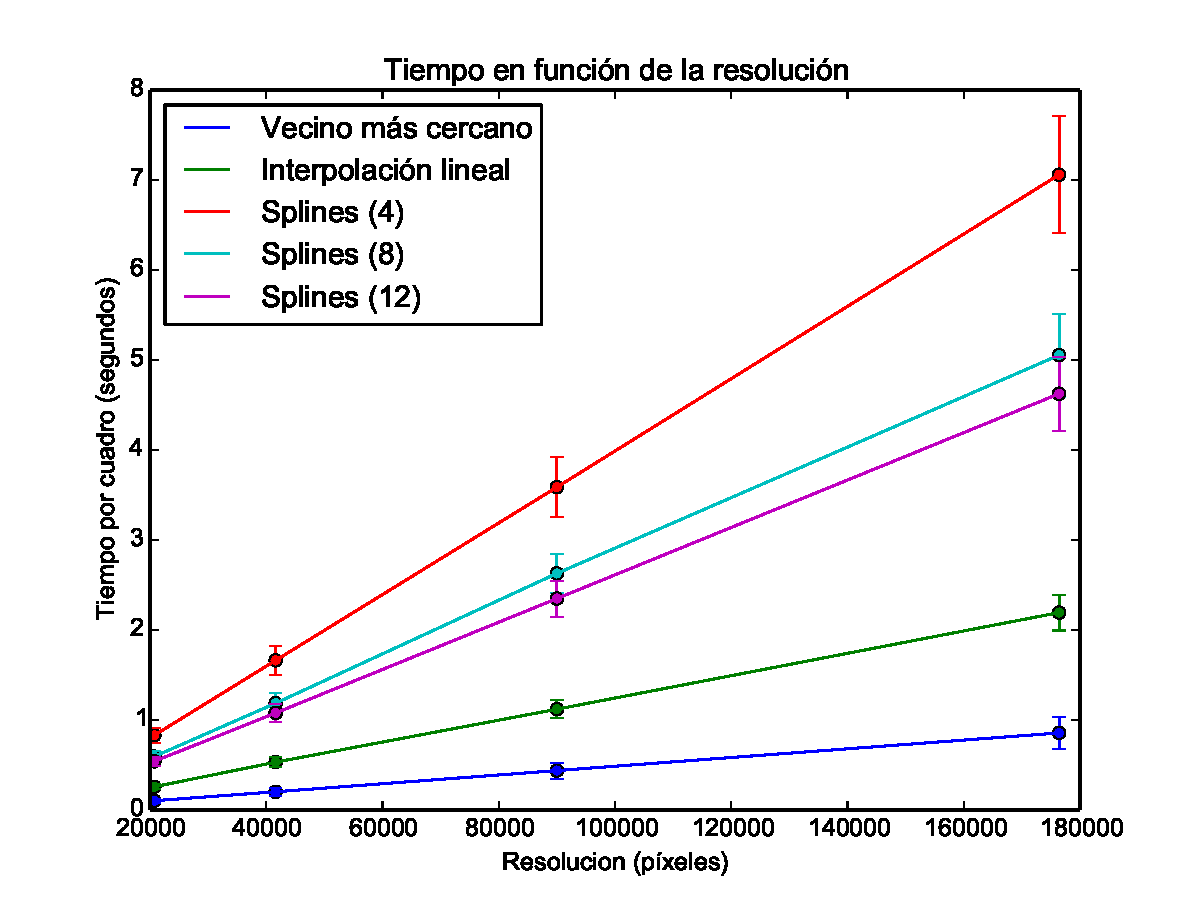
\includegraphics[width=0.7\textwidth]{imgs/resultados_tiempos/resolucion.pdf}
	\caption{\footnotesize Tiempo que se requiere al aplicar cada método sobre un video para interpolar 2 cuadros en función de la resolución del mismo. Los puntos representan la media 0.20-podada de cada muestra. Las barras verticales indican la varianza.}
	\label{fig:times-resolucion}
\end{figure}
\newpage
\subsection{Análisis cuantitativo del error}

Antes de ver los resultados, hagamos un análisis de los casos de prueba que tendremos en cuenta.

\begin{itemize}
    \item \texttt{darthvader}. El primer video contiene una cámara fija y un objeto moviendose a una velocidad relativamente lenta, con su entorno quieto. 
    \item \texttt{ff6}. Este es un video que contiene (a pesar de su corta duración), 6 tomas en escenarios totalmente distintos. Algunos escenarios presentan mucho movimiento, otros estan prácticamente quietos. Este es un video muy interesante para analizar porque es esperable que los algoritmos de interpolación en los que importa sobre todo información local (vecinos más cercanos, interpolación lineal fragmentaria) funcionen mejor que aquellos que toman información global (splines). Analizaremos todo esto más adelante. 
    \item \texttt{motocross}. En este video la cámara se mueve a gran velocidad, siguiendo a un objeto (una moto) que se encuentra más o menos centrada a lo largo de todo el video. El escenario que rodea a la moto se mueve en muy rápidamente.
    \item \texttt{penal}. En este video la cámara esta nuevamente fija, pero ahora hay un objeto que se mueve a velocidad medianemente rápida (pateador y arquero) y otro objeto que se mueve a una velocidad muy alta (pelota); mientras que todo el entorno se encuentra quieto. 
\end{itemize}

Elegimos estos videos porque creemos que representan las posibles situaciones o combinaciones que puede presentar un video de la vida real. No elegimos videos confeccionados a mano para analizar casos borde o extremos porque creemos que el análisis más interesante que se puede hacer está al rededor de casos reales, que son finalmente sobre los cuales se aplicarán estos algoritmos.

La métodología de experimentación fue la siguiente: extrajimos 1,2,4 u 8 cuadros por medio de cada video (utilizando el script \texttt{videoToTextfile.py}) y luego lo interpolamos con nuestros algoritmos. Finalmente, utilizando un script hecho por nosotros, comparamos los valores de los píxeles del video original contra los interpolados por nosotros. 

Elegimos esa cantidad de cuadros porque más de 8 cuadros se torna demasiado para interpolar, dado que se pierden muchos detalles del video original y el error se torna realmente alto (ya sucede eso con 8 cuadros).

Por último, para analizar el algoritmo de Splines utilizamos bloques de 4, 8 y 12 cuadros porque, nuevamente, si los bloques eran más grandes el video comenzaba a tener importantes artifacts (lo analizaremos más adelante, cuando analicemos cualitativamente los resultados) y entonces nos pareció adecuado poner 12 como el tamaño máximo de bloque a tomar (ya en algunos videos 12 es demasiado y el resultado es de mala calidad). Esto se debe a la localidad vs. globalidad de la que hablamos antes, dado que si un los frames de un video cambian mucho a lo largo del tiempo, tomar en cuenta frames lejanos a la hora de interpolar es contraproducente.

Sin más aclaraciones que hacer, pasemos a ver y analizar los resultados que obtuvimos.


\begin{figure}[H]
\centering
\begin{minipage}{0.35\textwidth}
    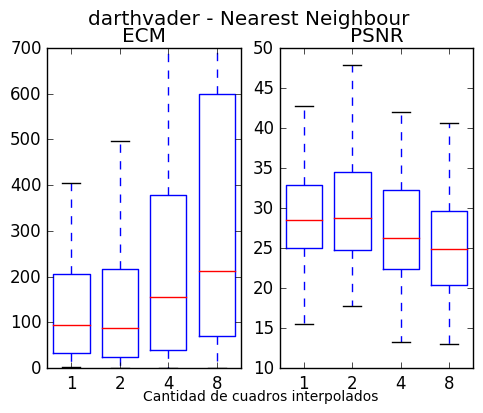
\includegraphics[width=1\textwidth]{imgs/resultados_error/darthvader_0.png}
\end{minipage}%
\begin{minipage}{0.35\textwidth}   
    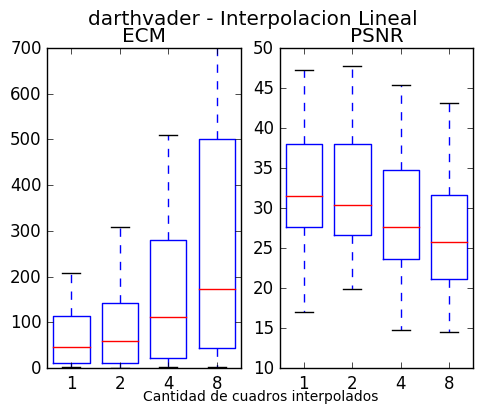
\includegraphics[width=1\textwidth]{imgs/resultados_error/darthvader_1.png} 
\end{minipage}
\end{figure}
\begin{figure}[H]
\centering
\begin{minipage}{0.33\textwidth}   
    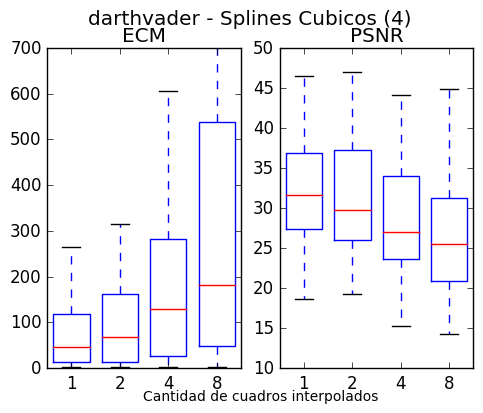
\includegraphics[width=1\textwidth]{imgs/resultados_error/darthvader_2.png} 
\end{minipage}\hfill
\begin{minipage}{0.33\textwidth}   
    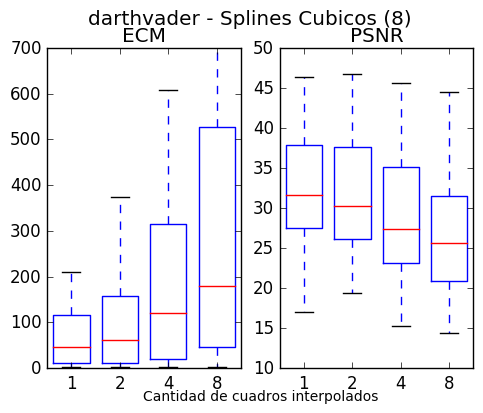
\includegraphics[width=1\textwidth]{imgs/resultados_error/darthvader_3.png} 
\end{minipage}\hfill
\begin{minipage}{0.33\textwidth}   
    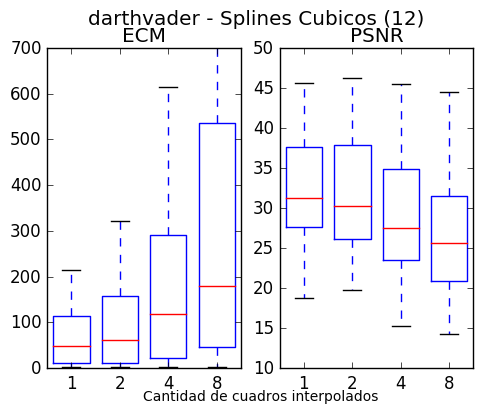
\includegraphics[width=1\textwidth]{imgs/resultados_error/darthvader_4.png} 
\end{minipage}
\label{fig:errdarthvader}
\caption{\footnotesize Resultados del cálculo de ECM y PSNR para cada algoritmo en el video \texttt{darthvader}. Para Splines cúbicos se indica además el tamaño de los bloques utilizados.}
\end{figure}


\begin{figure}[H]
\centering
\begin{minipage}{0.35\textwidth}
    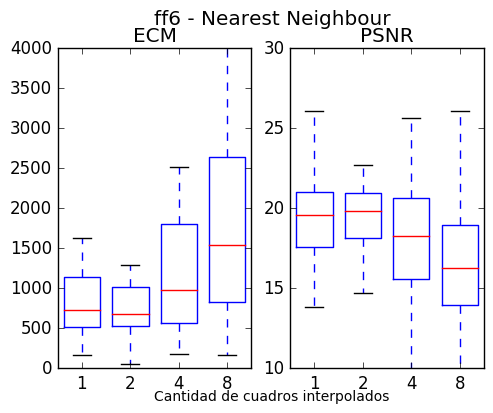
\includegraphics[width=1\textwidth]{imgs/resultados_error/ff6_0.png}
\end{minipage}%
\begin{minipage}{0.35\textwidth}   
    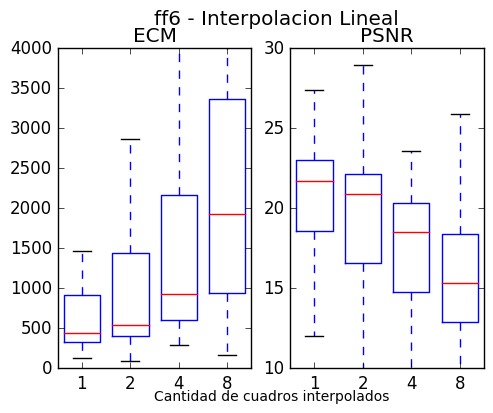
\includegraphics[width=1\textwidth]{imgs/resultados_error/ff6_1.png} 
\end{minipage}
\end{figure}
\begin{figure}[H]
\centering
\begin{minipage}{0.33\textwidth}   
    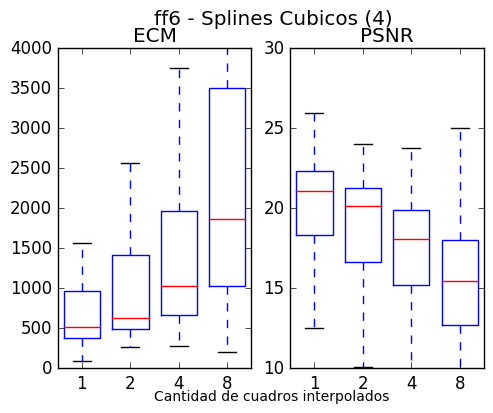
\includegraphics[width=1\textwidth]{imgs/resultados_error/ff6_2.png} 
\end{minipage}\hfill
\begin{minipage}{0.33\textwidth}   
    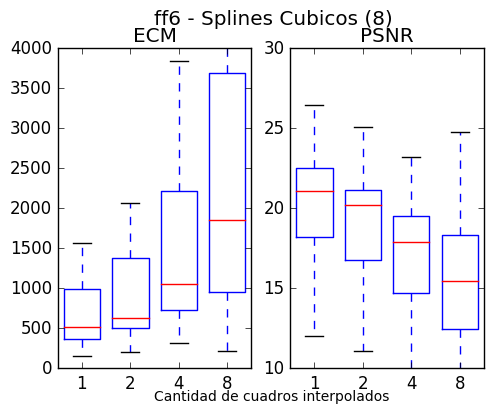
\includegraphics[width=1\textwidth]{imgs/resultados_error/ff6_3.png} 
\end{minipage}\hfill
\begin{minipage}{0.33\textwidth}   
    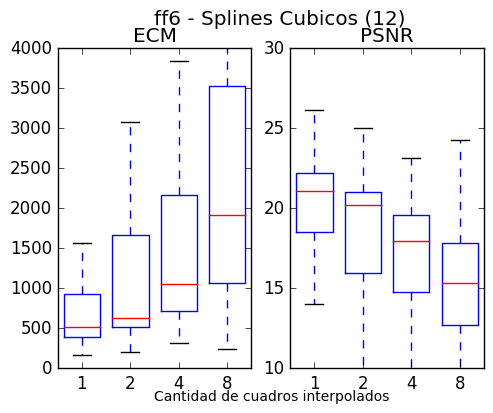
\includegraphics[width=1\textwidth]{imgs/resultados_error/ff6_4.png} 
\end{minipage}
\label{fig:errff6}
\caption{\footnotesize Resultados del cálculo de ECM y PSNR para cada algoritmo en el video \texttt{ff6}. Para Splines cúbicos se indica además el tamaño de los bloques utilizados.}
\end{figure}


\begin{figure}[H]
\centering
\begin{minipage}{0.35\textwidth}
    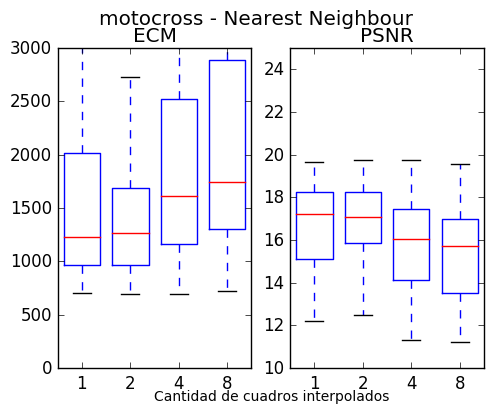
\includegraphics[width=1\textwidth]{imgs/resultados_error/motocross_0.png}
\end{minipage}%
\begin{minipage}{0.35\textwidth}   
    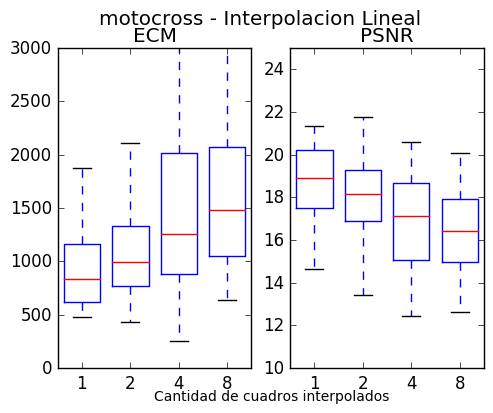
\includegraphics[width=1\textwidth]{imgs/resultados_error/motocross_1.png} 
\end{minipage}
\end{figure}
\begin{figure}[H]
\centering
\begin{minipage}{0.33\textwidth}   
    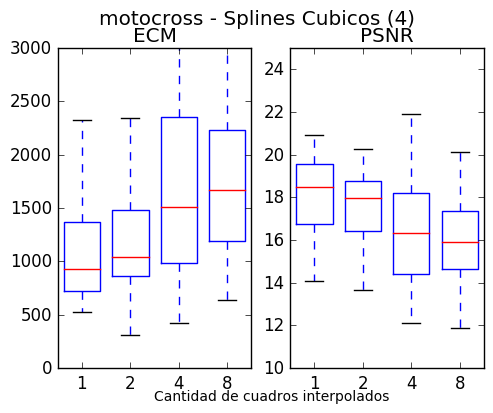
\includegraphics[width=1\textwidth]{imgs/resultados_error/motocross_2.png} 
\end{minipage}\hfill
\begin{minipage}{0.33\textwidth}   
    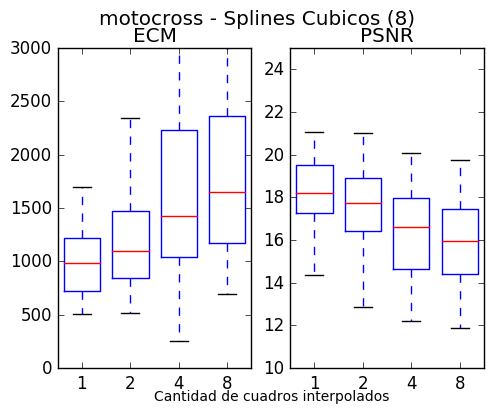
\includegraphics[width=1\textwidth]{imgs/resultados_error/motocross_3.png} 
\end{minipage}\hfill
\begin{minipage}{0.33\textwidth}   
    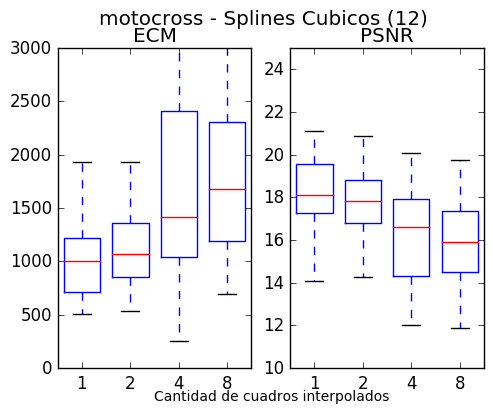
\includegraphics[width=1\textwidth]{imgs/resultados_error/motocross_4.png} 
\end{minipage}
\label{fig:errmotocross}
\caption{\footnotesize Resultados del cálculo de ECM y PSNR para cada algoritmo en el video \texttt{motocross}. Para Splines cúbicos se indica además el tamaño de los bloques utilizados.}
\end{figure}


\begin{figure}[H]
\centering
\begin{minipage}{0.35\textwidth}
    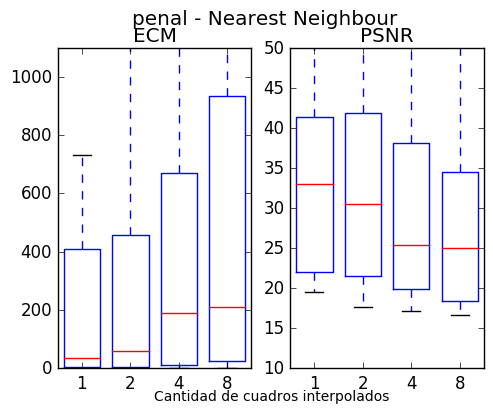
\includegraphics[width=1\textwidth]{imgs/resultados_error/penal_0.png}
\end{minipage}%
\begin{minipage}{0.35\textwidth}   
    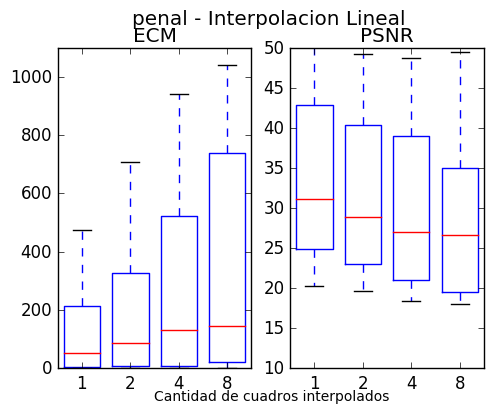
\includegraphics[width=1\textwidth]{imgs/resultados_error/penal_1.png} 
\end{minipage}
\end{figure}
\begin{figure}[H]
\centering
\begin{minipage}{0.33\textwidth}   
    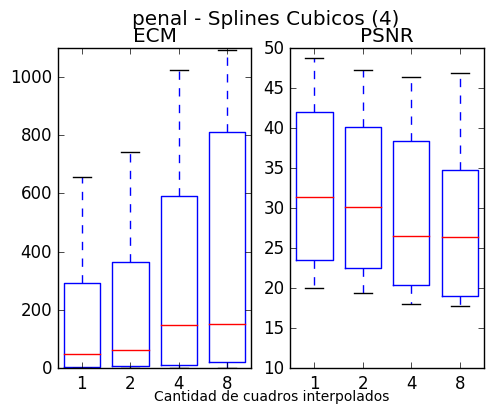
\includegraphics[width=1\textwidth]{imgs/resultados_error/penal_2.png} 
\end{minipage}\hfill
\begin{minipage}{0.33\textwidth}   
    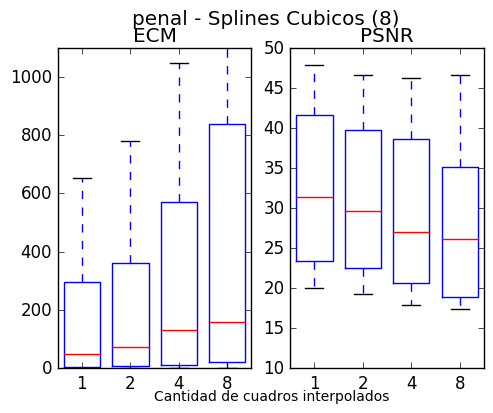
\includegraphics[width=1\textwidth]{imgs/resultados_error/penal_3.png} 
\end{minipage}\hfill
\begin{minipage}{0.33\textwidth}   
    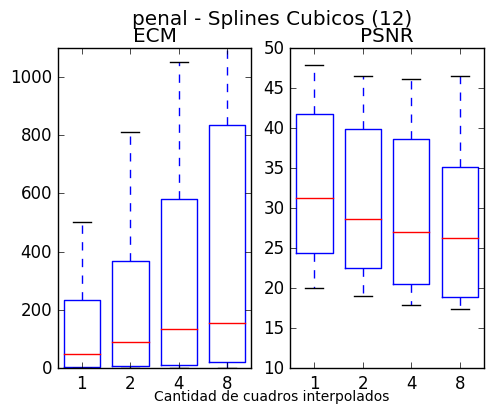
\includegraphics[width=1\textwidth]{imgs/resultados_error/penal_4.png} 
\end{minipage}
\label{fig:errpenal}
\caption{\footnotesize Resultados del cálculo de ECM y PSNR para cada algoritmo en el video \texttt{penal}. Para Splines cúbicos se indica además el tamaño de los bloques utilizados.}
\end{figure}

Antes de analizar los resultados, vale la pena explicar los gráficos que aparecen en las páginas anteriores. Cada boxplot representa los errores (en ECM y PSNR respectivamente) de todos los frames del video. Luego analizaremos dentro de cada video porqu\'e a veces el error es más alto y porqu\'e es más bajo, pero para este análisis en general nos bastará con los boxplots.

\subsubsection{\texttt{darthvader}}

Lo primero que podemos notar (muy esperable) es que el error aumenta cuando se intentan interpolar más cuadros. Esto se debe a que se intenta obtener más cantidad de cuadros a partir de una cantidad de datos menor, lo cual obviamente deteriorará la calidad del video.

Lo segundo que notamos es que, mientras el algoritmo de nearest neighbour tiene un error relativamente grande, los algoritmos de interpolación lineal y splines cúbicos (con todos los tamaños de bloque) presentan resultados muy similares. 
Creemos que esto se debe a la lentitud con la que transcurren los hechos en el video provoca que cualquier interpolación razonable de los valores de buenos resultados. 


\subsubsection{\texttt{ff6}}

En este caso, al igual que antes y al igual que en todos los videos que analizaremos, el error aumenta cuando se intentan interpolar más cuadros.


A diferencia que en el video anterior, en este caso se nota una diferencia entre los m\'etodos que utilizamos. Nearest neighbour, como siempre, es el peor, teniendo errores muy altos (dado que los cambios de escenarios en este video son bruscos, un frame puede no tener nada que ver con su anterior).


Luego, podemos ver que la interpolación lineal tuvo mejor performance que los splines cúbicos. La razón de eso es probablemente que, al ser un video que tiene cambios muy abrutpos de escenarios, es mucho mejor obtener los cuadros interpolados con la información lo más local posible, dado que cuadros lejanos tienen muy poco que ver.

Sin embargo, cuantos cuadros se tomen en el spline no afecta demasiado al error. Esto puede explicarse porque los escenarios son relativamente inmóviles, entonces la cantidad de cuadros que se tomen (mientras sean acotados) no debería afectar demasiado porque no agregan información nueva.

\subsubsection{\texttt{motocross}}

Como siempre, el error aumenta cuando se intentan interpolar más cuadros.

En este video sucede algo similar al anterior. Nearest neighbour es el peor porque el video se mueve muy rápido, un frame tiene poco que ver con el anterior. Nuevamente, la interpolación lineal tuvo mejor performance que los splines cúbicos. La razón de esto es la misma que la de antes: al ser un video que se mueve muy rápido, es mejor interpolar con información local que con información global.

Finalmente, podemos notar una diferencia con el video anterior. Podemos observar en la figura \ref{fig:errmotocross} como a más grande es el bloque que se toma para hacer splines cúbicos, más grande es el error. Puede verse que para un tamaño de bloque de 4 frames, el error cuadrático medio es aproximadamente 900, para un bloque de 8 frames de 950 y para uno de 12 es de 1000. 


Este hecho justifica nuestra explicación de porque en el video \texttt{ff6} el tamaño de los bloques no afectó tanto, dado que en este caso tomar bloques más grandes sí agrega nueva información, que sin embargo es perjudicial para el resultado, porque como todo se mueve muy rapidamente, la información nueva altera y distorsiona los resultados.

\subsubsection{\texttt{penal}}

Este es un video muy interesante para analizar. Primero, recordemos que en todo momento la mayor parte del video se encuentra quieta, mientras que algunos objetios que ocupan poca parte de la pantalla se mueven. 

Esto produce que (cuando hay que interpolar 1 o 2 cuadros) el error cuadrático medio se minimice con el algoritmo de vecino más cercano. Esto se debe a que como la mayor parte del video esta quieta, al interpolar con vecino mas cercanos, nos aseguramos que el error en estos lugares sea mínimo, y en las regiones del video que se mueven, el error tambi\'en será relativamente pequeño.

Además, al interpolar 1 o 2 cuadros, el error al usar splines (con cualquier tamaño de bloques) es menor que el de interpolación lineal. Una posible explicación para esto es que splines se adapta mejor que la interpolación lineal fragmentaria a los movimientos rápidos del video, manteniendo la exactitud de los pixeles que cambian poco, con lo cual puede sacarle ventaja.

Ahora bien, cuando se intentan interpolar 4 u 8 cuadros, la situación es muy distinta. Aquí el error de el algoritmo nearest neighbour sube mucho, sobrepasando al de interpolación lineal y splines cúbicos, que estan prácticamente empatados.

Explicar esto no es dificil: al tener que interpolar más cuadros, nearest neighbour empieza a aumentar su error dado que repetir un cuadro muchas conlleva bastante error en las partes del video de alto movimiento, dado que el error se arrastra por muchos cuadros. Los algoritmos de interpolación lineal y splines, al utilizar la información mas inteligentemente, son mas resilientes a la falta de información, lo cual les permite sobrepasar en rendimiento (con respecto al error) al
algoritmo de nearest neighbour cuando hay que interpolar muchos cuadros.



\newpage
\subsection{Análisis cualitativo de los métodos}

En esta sección nos concentraremos en las caracteristicas de los métodos utilizados que escapan a nuestros análisis anteriores. Si bien logramos tener una idea de la complejidad temporal y el nivel de error que pueden tener los videos que generamos aun no vimos con suficiente claridad los efectos particulares que pueden llegar a porducirse, qué tipo de errores pueden haber y cómo varian entre los distintos métodos. Esto es de lo que hablaremos en esta sección.

Un video esta formado por una sucesión finita de imagenes, al reproducirlo se pasa de una imagen a la siguiente lo cual puede causar cambios en los valores de los pixels que se estan visualizando. La interpolación se basara en esos pixels para calcular nuevas imagenes que se agregaran al video, en esta sección veremos de que forma el grado de cambio entre los pixels puede afectar la calidad del video resultante tras la interpolación.

Todos los videos sobre los que trabajaremos aquí seran el resultado de aplicar alguno de los métodos de interpolación sobre los pocos videos base que describimos previamente, se detallaran siempre los métodos utilizados de forma que los experimentos realizados puedan replicarse facilmente.

Nuestra primer hipótesis es que según la forma en que varían los pixels en el video podrían presentarse mayores dificultades y errores al intentar pasarlo a camara lenta. Por lo tanto lo que haremos en esta sección sera dividir los experimentos en cuatro tipos de video base y analizar cada caso particular con los métodos propuestos. Escogimos 4 ejemplares distintos, un por cada categoría de video que nos pareció relevante analizar. Para cada video hicimos experimentos con cada método interpolando 1, 2, 4 y 8 cuadros. Se presentarán en esta sección los casos mas representativos de nuestros hallazgos.

\subsubsection{Video de control}

En los próximos experimentos analizaremos videos con movimientos rápidos de objetos y cámara intentando verificar ciertas ideas sobre posibles artifacts que podrian generarse. Antes de eso utilizaremos un video de control el cual no presenta ninguna de esas caracteristicas, este será un video con movimiento relajado el cual nos permitira verificar como se comportan los métodos con videos que, según creemos, no presentaran problemas para luego compararlos con los casos mas problemáticos. El caso mas trivial sería un video completamente estático. Pero se ve facilmente al analizar el funcionamiento de nuestros métodos que el resultado sera un video tambien estático pero de mayor duración, lo cual cumpliría correctamente el resultado deseado. Un caso un poco mas interesante y el cual utilizaremos como video de control es el caso en que hay cierto movimiento pero nada de gran velocidad.

Como video seleccionamos una toma de la carrera de un grupo de babosas.

\begin{figure}[H]
\centering
\begin{minipage}{0.60\textwidth}   
    \fbox{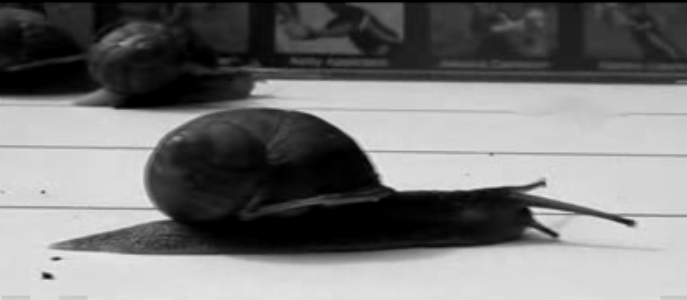
\includegraphics[width=1\textwidth]{imgs/cualitativos/babosa.png}}
\end{minipage}\hfill
\caption{\footnotesize Captura del video babosa.avi con el cuadruple de cuadros de lo normal calculados utilizando splines de bloque de radio 4, no se nota en ningún momento algún artifact significativo.}
\end{figure}

Al ver los resultados se corroboró que utilizando splines y interpolación lineal no habian problemas y el video resultante tenia un buen efecto de camara lenta, solo se notaron partes borrosas en las antenas, creemos que debido a que estas producen los movimientos mas rápidos en el video. Con Nearest Neighbour la historia es distinta, al agregar mas de 2 cuadros al video original comienza a perder mucha fluidés, agregando 8 cuadros el video ya carece completamente de un movimiento natural, esta caracteristica creemos que persistirá siempre al utilizar este método.

\subsubsection{Movimiento rápido de cámara}

Un caso que nos pareció relevante es el de los videos que tienen movimientos rápidos de cámara, como ejemplar de esta situación utilizamos al video nombrado previamente \textit{motocross}. Para este caso volvió a ocurrir con \textit{Nearest Neighbour} que la imagen perdia fluidez a medida que se intentaban agregar mas cuadros. Para  \textit{Splines} e \textit{Interpolación Lineal}  sucedió lo esperado, los movimientos rapidos del video produjeron efectos indeseados, los cuales empeoraban a medida que se agregaban mas cuadros. El error puede observarse en la imagen de la izquierda.

\begin{figure}[H]
\centering
\begin{minipage}{0.48\textwidth}
    \fbox{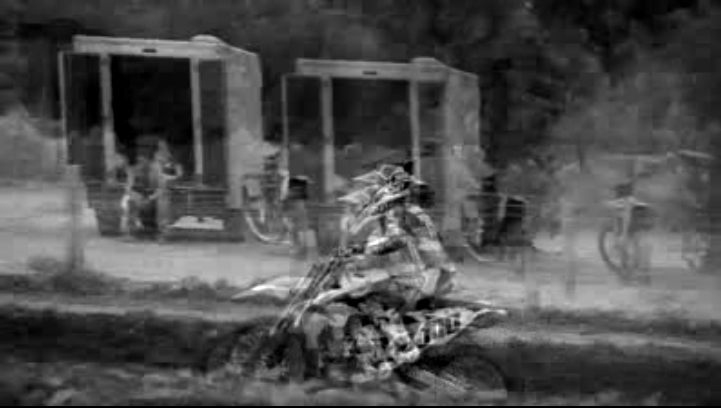
\includegraphics[width=1\textwidth]{imgs/cualitativos/motocross_1.png}}
\end{minipage}%
\hfill
\begin{minipage}{0.48\textwidth}   
    \fbox{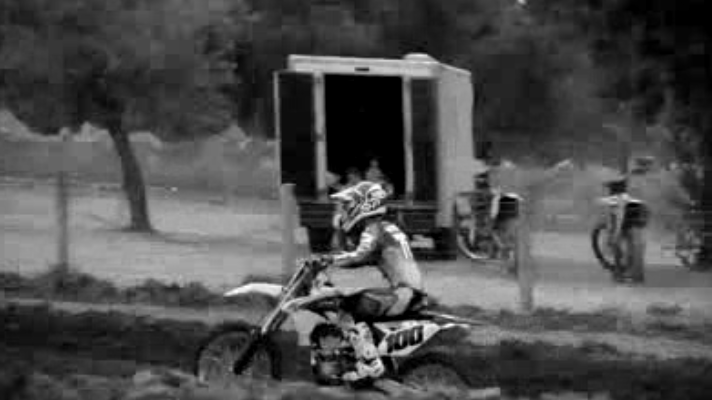
\includegraphics[width=1\textwidth]{imgs/cualitativos/motocross_2.png}}

\end{minipage}
\caption{\footnotesize A la izquierda se tiene el resultado de un cuadro calculado con Splines al interpolar de a 4 cuadros con bloques de radio 4, se observa una superposición importante entre dos imagenes. En la izquierda se ve una toma del video original}
\end{figure}

Lo que sucede es que debido al gran ritmo de cambio entre cada fotograma los cuadros que se agregan al video se calculan basados en imagenes muy distintas, los métodos que utilizamos no son suficientemente buenos para predecir el cuadro adecuado y en concecuencia fallan en dar una imagen intermedia adecuada.

Otra observación que hicimos en este video fue que a simple vista no parece haber diferencia significativa entre los resultados de Splines e interpolación lineal, ambos funcionan correctamente al agregar 1 y 2 cuadros y comienzan a fallar a un ritmo similar al comenzar a agregar mas cuadros. 

\subsubsection{Movimiento rápido de objetos}

Para este experimento utilizamos el video \textit{penal}, este se puede ver como un caso particular del anterior. Ya que hay movimiento rapido de pixels por lo que se presentan los mismos inconvenientes pero solo sobre un pequeño conjunto de pixels, los que estan en la trayectoria de la pelota y el jugador, en ese espacio es donde al utilizar splines y lineal se espera experimentar al igual que en el caso anterior un efecto de transparencia y superposición indeseable entre el fondo y el lugar donde estuvo el objeto previamente.


\begin{figure}[H]
\centering
\begin{minipage}{0.48\textwidth}
    \fbox{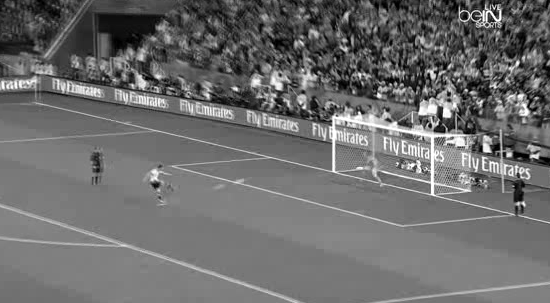
\includegraphics[width=1\textwidth]{imgs/cualitativos/penal_1.png}}
\end{minipage}%
\hfill
\begin{minipage}{0.48\textwidth}   
    \fbox{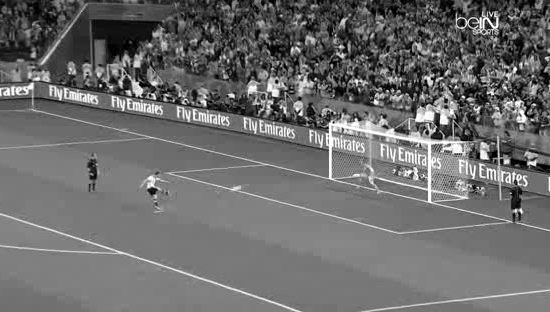
\includegraphics[width=1\textwidth]{imgs/cualitativos/penal_2.png}}

\end{minipage}
\caption{\footnotesize A la izquierda se tiene el resultado de un fotograma calculado con Splines agregando 8 cuadros con bloques de radio 4, se observa una superposición importante entre cuadros. A la derecha esta una toma del video original}
\end{figure}


Al ver los videos se corrobora lo esperado. El artifact visto en la figura aumenta cuanto mayor es la cantidad de cuadros que queremos agregar. Para \textit{Nearest Neighbour} el efecto no existe pero la imagen tiene movimientos muy bruscos y parece mas estática a medida que agregamos mas cuadros.

\subsubsection{Cambio de Cámara}

Los cambios de cámara creemos que serán los que produzcan los mayores problemas para Splines e interpolación lineal debido a que estos producen las mayores diferencias entre cuadros contiguos, creemos que aquí en algunos casos puede llegar a ser preferible incluso \textit{nearest neighbour} a pesar de su dinámica pobre. Para verificar nuestras ideas utilizamos el video \textit{ff6}.
También nos interesa comprobar lo charlado previamente en la sección de errores sobre que tanto afectara el tamaño de los bloques de los Splines, intentaremos ver si esto podria llegar a jugar un rol en que tan dramaticos son los artifacts.


\begin{figure}[H]
\centering
\begin{minipage}{0.31\textwidth}   
    \fbox{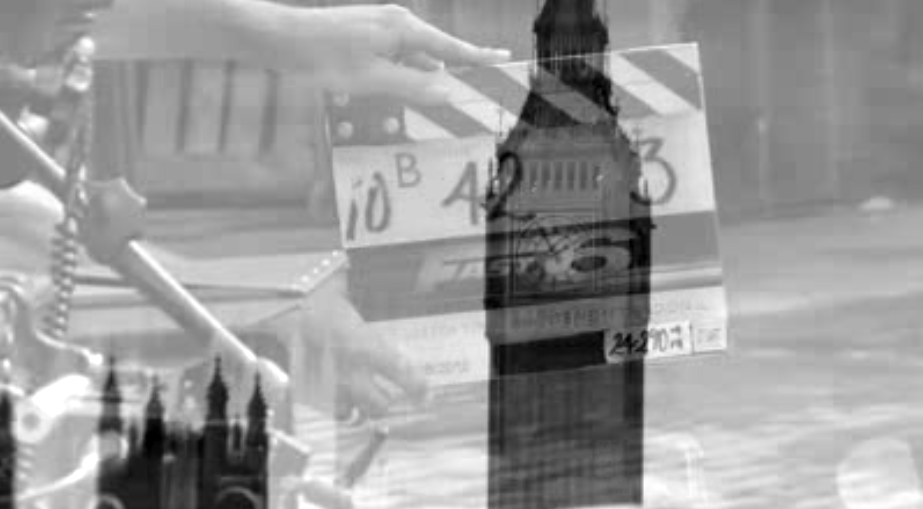
\includegraphics[width=1\textwidth]{imgs/cualitativos/ff6_1.png}}

\end{minipage}
\hfill
\begin{minipage}{0.31\textwidth}   
    \fbox{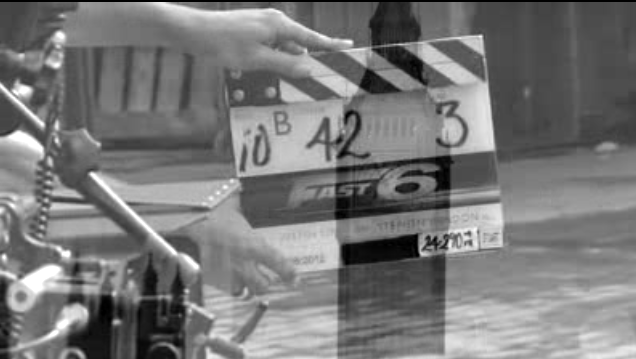
\includegraphics[width=1\textwidth]{imgs/cualitativos/ff6_2.png}}
\end{minipage}
\hfill
\begin{minipage}{0.31\textwidth}   
    \fbox{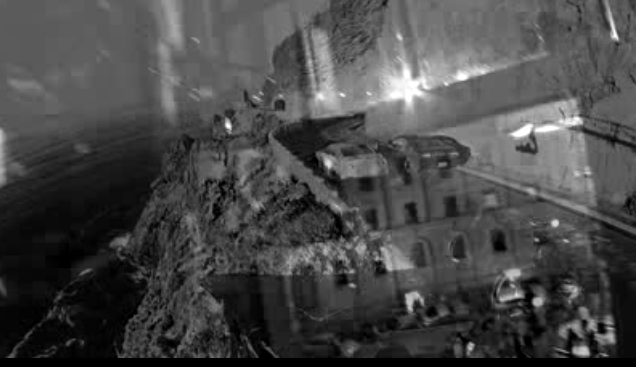
\includegraphics[width=1\textwidth]{imgs/cualitativos/ff6_3.png}}
\end{minipage}
\caption{\footnotesize Distintos artifacts producidos por Splines e Interpolación lineal interpolando 4 cuadros. El del medio es Splines cúbicos interpolando 4 cuadros con 8 de radio, los otros son interpolación lineal de 8 cuadros.}

\label{fig:ff6}

\end{figure}

\begin{figure}[H]
\centering
\begin{minipage}{0.31\textwidth}   
    \fbox{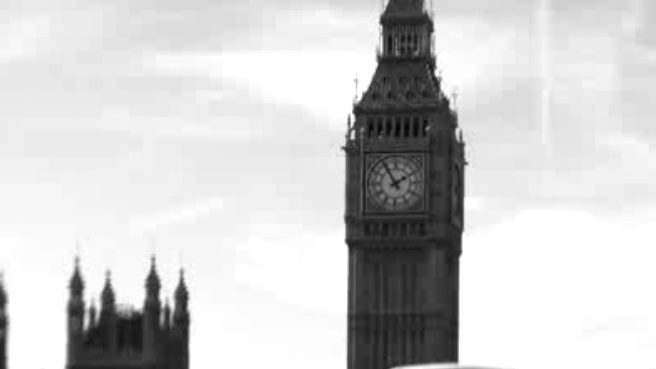
\includegraphics[width=1\textwidth]{imgs/cualitativos/ff6_4.png}}

\end{minipage}
\hfill
\begin{minipage}{0.31\textwidth}   
    \fbox{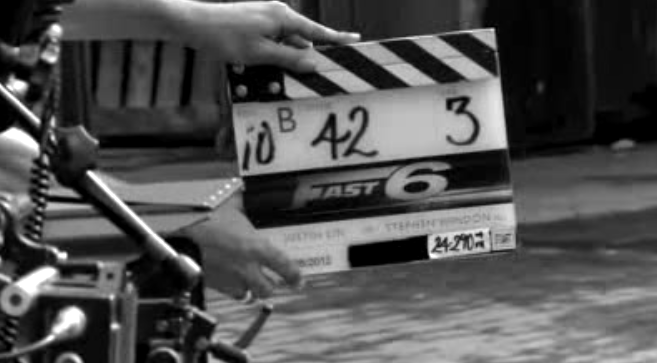
\includegraphics[width=1\textwidth]{imgs/cualitativos/ff6_7.png}}
\end{minipage}
\hfill
\begin{minipage}{0.31\textwidth}   
    \fbox{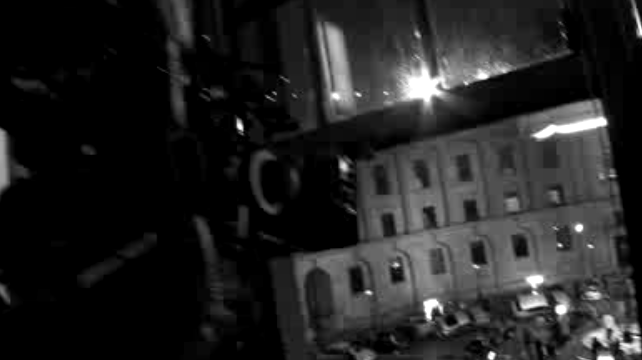
\includegraphics[width=1\textwidth]{imgs/cualitativos/ff6_6.png}}
\end{minipage}
\caption{\footnotesize Imagenes originales.}

\label{fig:ff6}

\end{figure}

Como se ve en las imagenes hay cuadros formados por imagenes totalmente distintas fusionadas lo cual produce un efecto indeseable. Estos problemas se ven a lo largo de todos los cambios de cámara del video. Se deduce de este experimento que no es buena idea intentar interpolar entre cambios de cámara, una posible solución podria ser trabajar sobre cada toma por separado, hacer la interpolación deseada y luego volver a unir los subvideos obtenidos, asi se evitaria generar cuadros entre tomas de lugares distintos.

Con respecto al tamaño de los bloques de Splines se pudo verificar lo charlado anteriormente en la sección de errores, con distintos tamaños de bloque (se utilizaron radios de 1, 2, 8 y 16) no se observaron cambios significativos.

Como observación final debemos decir que a simple vista no pudimos presenciar para ninguno de los casos analizados una diferencia demasiado abrupta entre interpolación lineal y Splines con distintos tamaños de bloques. Si bien en ciertas circunstancias habian mejoras con algunos de estos métodos respecto de los demás estas no superaban ampliamente a las demas y presentaban los mismos artifacts y decadencias para casos iguales de interpolación. Esta observación de seguro este relacionada con la calidad baja de los videos y la impresición del análisis a ojo por lo que quedara como trabajo a futuro la verificación y profundización de esta idea.

\newpage
\section{Conclusiones}
A continuación pasaremos en limpio las conclusiones que pudimos sacar con la realización del presente trabajo práctico. Dado que en la práctica las tres áreas de experimentación sobre las que realizamos nuestros análisis se entrelazan y son interdependientes, trataremos de que las conclusiones sean globales y no un mero enlistamiento de los resultados de cada sección. 

Vimos que en general interpolar con el método de vecino más cercano nunca da resultados mejores en términos de calidad que los otros métodos, pues carece de toda fluidez y entre más cuadros se desean agregar más notoriamente impacta esto. Si bien puede resultar ser el más rápido, la diferencia con el costo de usar interpolación lineal que presenta resultados más satisfactorios, no es demasiado grande, por lo que este casi siempre va a terminar siendo preferible. 

Entre la interpolación lineal y las tres variantes de splines cúbicos no se encontraron grandes diferencias de comportamiento en cuanto a la calidad de los videos producidos. Lineal tiende a ser un poco más sólida en los casos en que la cámara se mueve muy rápido pues depende de los frames inmediatos a interpolar (y por tanto que menos difieren), en contraposición a splines que requiere cuadros más alejados (lo que termina convirtiéndose en una \emph{desinformación} para el método). En esa línea, considerar bloques de tamaño 4 u 8 para splines resulta más robusto que tomar 12. Pero a su vez, los tiempos de splines con bloques de tamaño 4 aumentan tan vertiginosamente (especialmente en base a la cantidad de cuadros originales del video y su resolución) que en general no tiene sentido siquiera considerar esta opción.

Por lo tanto, de las tres variantes de splines la más razonable parece ser la que considera bloques de tamaño 8. Para videos donde no hay movimientos de cámara rápidos y los objetos se mueven a una velocidad normal (y aún habiendo algunos movimientos bruscos) este método da resultados un poco más fluidos que los de la interpolación lineal. No obstante el tiempo de cómputo a pagar sigue siendo sensiblemente más alto. Por lo tanto, debe escogerse el método que mejor ajuste a la situación: si hay movimientos abruptos de cámara o no, si se desea preprocesar el video del lado del servidor o si se quiere procesar durante el \textit{streaming} del lado del usuario.

Desde el punto de vista práctico propuesto en el trabajo, el cual proponía intentar pasar a cámara lenta videos normales para evitar sobrecargar una red con videos mas pesados de lo necesario, llegamos a la conclusión de que esto es posible aunque tiene ciertas limitaciones, ya que excepto para videos con cambios muy graduales en los valores de sus pixels, los métodos utilizados comienzan a presentar grandes falencias al intentar interpolar de a mas de 2 cuadros, a partir de esos valores no se considera que los videos resultantes tengan una calidad suficientemente buena para el contexto planteado, estos estarían demasiado alejados de una versión real de cámara lenta.

Como último punto a destacar, vimos que ninguno de nuestros métodos tolera bien los cambios de tomas. Llegamos a la conclusión de que lo mejor que se puede hacer ante esta situación es subdividir el video en las distintas tomas para luego interpolar con un método u otro cada subdivisión de manera independiente. El como implementar esto de manera eficiente queda como trabajo a futuro, aunque una primera aproximación sencilla sería simplemente ir recorriendo el video frame por frame, tomando la diferencia respecto del anterior (usando alguna métrica adecuada), y a partir de estos valores armar la partición de tomas.

\newpage

\section{Apéndices}

\newpage

\subsubsection{Videos de Referencia}
\label{sec:links}

Los videos originales utilizados, junto con algunos de los que generamos aplicando los distintos métodos de interpolación se pueden encontrar en el siguiente link: \url{http://bit.ly/1HuAwnj}\footnote{Este link es un acortamiento de \newline \url{https://drive.google.com/drive/folders/0B5hNK09AHoDcMExwZVNQVVI3Zkk}, por comodidad}.

% si se descomenta esto, aparecen todas las cosas de la bibliografia, hasta
% las que nunca fueron citadas en el TP. es una eleccion de diseño.
% \nocite{*}
\printbibliography



\end{document}
